% 图 7.13 (a) 交换劈裂双子带 g(E) (b) ↑/↓ 两支费米面同心圆 (c) q 增大时 k+q 空洞位置序列 (d) Stoner 连续谱与自旋波支
\documentclass[tikz,border=5pt]{standalone}
\usetikzlibrary{arrows.meta}
\usepackage{amsmath}
\usepackage{bm}
\usepackage{fontspec}
\setmainfont{Times New Roman}
\begin{document}
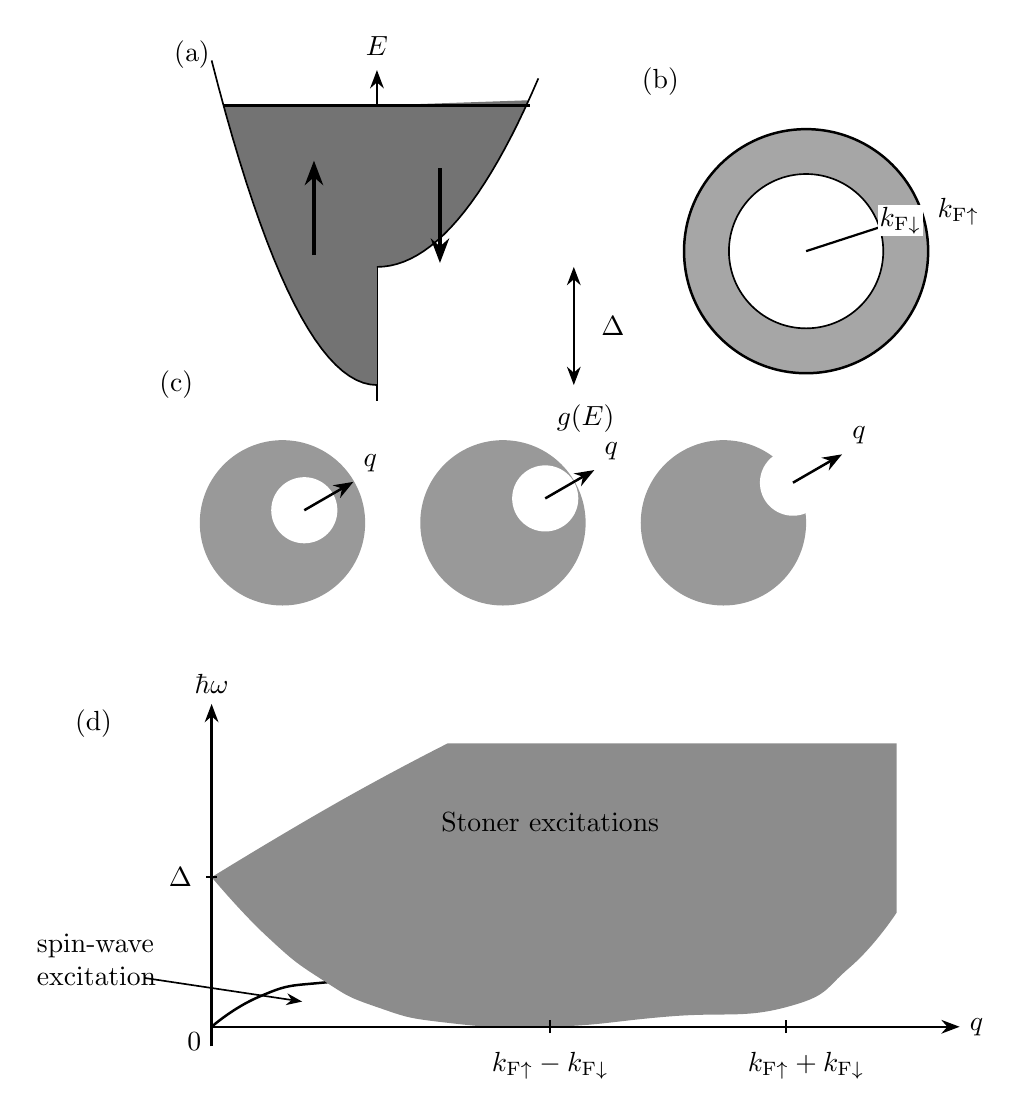
\begin{tikzpicture}[line width=0.8pt,>=Stealth]
% ---------- (a) 双子带 ----------
\begin{scope}
\node at (0.35,4.75) {(a)};
% 中央 E 轴
\draw[->] (2.7,0.35) -- (2.7,4.55);
\node[above] at (2.7,4.6) {$E$};
% 左带（↑）：顶点 (2.7,0.55)，填充至 4.1
\fill[black!55] plot[domain=0:1.949] (2.7-\x,{0.55+0.935*\x*\x}) -- (2.7,4.1) -- cycle;
\draw[line width=0.6pt] plot[domain=0:2.1] (2.7-\x,{0.55+0.935*\x*\x});
% 右带（↓）：顶点 (2.7,2.05)
\fill[black!55] plot[domain=0:1.927] (2.7+\x,{2.05+0.57*\x*\x}) -- (2.7,4.1) -- cycle;
\draw[line width=0.6pt] plot[domain=0:2.05] (2.7+\x,{2.05+0.57*\x*\x});
\draw[line width=0.9pt] (0.76,4.1) -- (4.64,4.1);
% 自旋箭头
\draw[line width=1.3pt,->] (1.9,2.2) -- (1.9,3.4);
\draw[line width=1.3pt,->] (3.5,3.3) -- (3.5,2.1);
% Δ 双箭头
\draw[Stealth-Stealth] (5.2,0.55) -- (5.2,2.05);
\node[right] at (5.42,1.3) {$\Delta$};
\node at (5.35,0.12) {$g(E)$};
\end{scope}
% ---------- (b) 双同心圆 ----------
\begin{scope}[shift={(8.15,2.25)}]
\node at (-1.85,2.15) {(b)};
\fill[even odd rule,black!35] (0,0) circle (1.55) (0,0) circle (0.98);
\draw[line width=0.9pt] (0,0) circle (1.55);
\draw[line width=0.6pt] (0,0) circle (0.98);
% 半径箭头与标注
\draw[->] (0,0) -- (18:1.55);
\node[fill=white,inner sep=0.8pt] at (18:1.26) {$k_{\mathrm{F}\downarrow}$};
\node[right] at (18:1.62) {$k_{\mathrm{F}\uparrow}$};
\end{scope}
% ---------- (c) q 增大序列 ----------
\begin{scope}[shift={(0,-1.2)}]
\node at (0.15,1.75) {(c)};
\foreach \cx/\off in {1.5/0.32, 4.3/0.62, 7.1/1.02}{
  \fill[black!40] (\cx,0) circle (1.05);
  \fill[white] ({\cx+\off*cos(30)},{\off*sin(30)}) circle (0.42);
  \draw[->,line width=0.9pt]
    ({\cx+\off*cos(30)},{\off*sin(30)}) --
    ({\cx+\off*cos(30)+0.72*cos(30)},{\off*sin(30)+0.72*sin(30)});
  \node[above right] at ({\cx+\off*cos(30)+0.72*cos(30)},
                         {\off*sin(30)+0.72*sin(30)}) {$q$};
}
\end{scope}
% ---------- (d) Stoner 连续谱 ----------
\begin{scope}[shift={(0.6,-7.6)}]
% 自旋波支（先画，超出部分被连续谱覆盖）
\draw[line width=0.9pt] plot[smooth,tension=0.9] coordinates
  {(0,0) (0.6,0.38) (1.3,0.55) (2.0,0.5) (3.0,0.15)};
% 连续谱灰区
\fill[black!45] plot[smooth,tension=0.85] coordinates
  {(0,1.9) (0.7,1.15) (1.4,0.6) (2.1,0.25) (3.0,0.05) (4.3,0.0) (5.8,0.13) (7.3,0.25) (8.1,0.75) (8.7,1.45)}
  -- (8.7,3.6) -- (3.0,3.6)
  plot[smooth,tension=0.9] coordinates {(3.0,3.6) (1.6,2.85) (0,1.9)};
\node at (4.3,2.6) {Stoner excitations};
% 轴
\draw[->] (0,-0.25) -- (0,4.1) node[above] {$\hbar\omega$};
\draw[->] (0,0) -- (9.5,0) node[right] {$q$};
\node[below left] at (0,0.05) {$0$};
% Δ 与 q 轴刻度
\draw[line width=0.7pt] (-0.07,1.9) -- (0.07,1.9);
\node[left] at (-0.12,1.9) {$\Delta$};
\draw[line width=0.7pt] (4.3,-0.08) -- (4.3,0.08);
\draw[line width=0.7pt] (7.3,-0.08) -- (7.3,0.08);
\node at (4.3,-0.5) {$k_{\mathrm{F}\uparrow}-k_{\mathrm{F}\downarrow}$};
\node at (7.55,-0.5) {$k_{\mathrm{F}\uparrow}+k_{\mathrm{F}\downarrow}$};
% spin-wave 标签与指向箭头
\node[align=left,anchor=west] at (-2.35,0.85) {spin-wave\\excitation};
\draw[->,line width=0.6pt] (-0.85,0.62) -- (1.15,0.32);
% (d) 标签
\node at (-1.5,3.85) {(d)};
\end{scope}
\end{tikzpicture}
\end{document}
